% Options for packages loaded elsewhere
\PassOptionsToPackage{unicode}{hyperref}
\PassOptionsToPackage{hyphens}{url}
%
\documentclass[
]{book}
\usepackage{amsmath,amssymb}
\usepackage{iftex}
\ifPDFTeX
  \usepackage[T1]{fontenc}
  \usepackage[utf8]{inputenc}
  \usepackage{textcomp} % provide euro and other symbols
\else % if luatex or xetex
  \usepackage{unicode-math} % this also loads fontspec
  \defaultfontfeatures{Scale=MatchLowercase}
  \defaultfontfeatures[\rmfamily]{Ligatures=TeX,Scale=1}
\fi
\usepackage{lmodern}
\ifPDFTeX\else
  % xetex/luatex font selection
\fi
% Use upquote if available, for straight quotes in verbatim environments
\IfFileExists{upquote.sty}{\usepackage{upquote}}{}
\IfFileExists{microtype.sty}{% use microtype if available
  \usepackage[]{microtype}
  \UseMicrotypeSet[protrusion]{basicmath} % disable protrusion for tt fonts
}{}
\makeatletter
\@ifundefined{KOMAClassName}{% if non-KOMA class
  \IfFileExists{parskip.sty}{%
    \usepackage{parskip}
  }{% else
    \setlength{\parindent}{0pt}
    \setlength{\parskip}{6pt plus 2pt minus 1pt}}
}{% if KOMA class
  \KOMAoptions{parskip=half}}
\makeatother
\usepackage{xcolor}
\usepackage{color}
\usepackage{fancyvrb}
\newcommand{\VerbBar}{|}
\newcommand{\VERB}{\Verb[commandchars=\\\{\}]}
\DefineVerbatimEnvironment{Highlighting}{Verbatim}{commandchars=\\\{\}}
% Add ',fontsize=\small' for more characters per line
\usepackage{framed}
\definecolor{shadecolor}{RGB}{248,248,248}
\newenvironment{Shaded}{\begin{snugshade}}{\end{snugshade}}
\newcommand{\AlertTok}[1]{\textcolor[rgb]{0.94,0.16,0.16}{#1}}
\newcommand{\AnnotationTok}[1]{\textcolor[rgb]{0.56,0.35,0.01}{\textbf{\textit{#1}}}}
\newcommand{\AttributeTok}[1]{\textcolor[rgb]{0.13,0.29,0.53}{#1}}
\newcommand{\BaseNTok}[1]{\textcolor[rgb]{0.00,0.00,0.81}{#1}}
\newcommand{\BuiltInTok}[1]{#1}
\newcommand{\CharTok}[1]{\textcolor[rgb]{0.31,0.60,0.02}{#1}}
\newcommand{\CommentTok}[1]{\textcolor[rgb]{0.56,0.35,0.01}{\textit{#1}}}
\newcommand{\CommentVarTok}[1]{\textcolor[rgb]{0.56,0.35,0.01}{\textbf{\textit{#1}}}}
\newcommand{\ConstantTok}[1]{\textcolor[rgb]{0.56,0.35,0.01}{#1}}
\newcommand{\ControlFlowTok}[1]{\textcolor[rgb]{0.13,0.29,0.53}{\textbf{#1}}}
\newcommand{\DataTypeTok}[1]{\textcolor[rgb]{0.13,0.29,0.53}{#1}}
\newcommand{\DecValTok}[1]{\textcolor[rgb]{0.00,0.00,0.81}{#1}}
\newcommand{\DocumentationTok}[1]{\textcolor[rgb]{0.56,0.35,0.01}{\textbf{\textit{#1}}}}
\newcommand{\ErrorTok}[1]{\textcolor[rgb]{0.64,0.00,0.00}{\textbf{#1}}}
\newcommand{\ExtensionTok}[1]{#1}
\newcommand{\FloatTok}[1]{\textcolor[rgb]{0.00,0.00,0.81}{#1}}
\newcommand{\FunctionTok}[1]{\textcolor[rgb]{0.13,0.29,0.53}{\textbf{#1}}}
\newcommand{\ImportTok}[1]{#1}
\newcommand{\InformationTok}[1]{\textcolor[rgb]{0.56,0.35,0.01}{\textbf{\textit{#1}}}}
\newcommand{\KeywordTok}[1]{\textcolor[rgb]{0.13,0.29,0.53}{\textbf{#1}}}
\newcommand{\NormalTok}[1]{#1}
\newcommand{\OperatorTok}[1]{\textcolor[rgb]{0.81,0.36,0.00}{\textbf{#1}}}
\newcommand{\OtherTok}[1]{\textcolor[rgb]{0.56,0.35,0.01}{#1}}
\newcommand{\PreprocessorTok}[1]{\textcolor[rgb]{0.56,0.35,0.01}{\textit{#1}}}
\newcommand{\RegionMarkerTok}[1]{#1}
\newcommand{\SpecialCharTok}[1]{\textcolor[rgb]{0.81,0.36,0.00}{\textbf{#1}}}
\newcommand{\SpecialStringTok}[1]{\textcolor[rgb]{0.31,0.60,0.02}{#1}}
\newcommand{\StringTok}[1]{\textcolor[rgb]{0.31,0.60,0.02}{#1}}
\newcommand{\VariableTok}[1]{\textcolor[rgb]{0.00,0.00,0.00}{#1}}
\newcommand{\VerbatimStringTok}[1]{\textcolor[rgb]{0.31,0.60,0.02}{#1}}
\newcommand{\WarningTok}[1]{\textcolor[rgb]{0.56,0.35,0.01}{\textbf{\textit{#1}}}}
\usepackage{longtable,booktabs,array}
\usepackage{calc} % for calculating minipage widths
% Correct order of tables after \paragraph or \subparagraph
\usepackage{etoolbox}
\makeatletter
\patchcmd\longtable{\par}{\if@noskipsec\mbox{}\fi\par}{}{}
\makeatother
% Allow footnotes in longtable head/foot
\IfFileExists{footnotehyper.sty}{\usepackage{footnotehyper}}{\usepackage{footnote}}
\makesavenoteenv{longtable}
\usepackage{graphicx}
\makeatletter
\def\maxwidth{\ifdim\Gin@nat@width>\linewidth\linewidth\else\Gin@nat@width\fi}
\def\maxheight{\ifdim\Gin@nat@height>\textheight\textheight\else\Gin@nat@height\fi}
\makeatother
% Scale images if necessary, so that they will not overflow the page
% margins by default, and it is still possible to overwrite the defaults
% using explicit options in \includegraphics[width, height, ...]{}
\setkeys{Gin}{width=\maxwidth,height=\maxheight,keepaspectratio}
% Set default figure placement to htbp
\makeatletter
\def\fps@figure{htbp}
\makeatother
\setlength{\emergencystretch}{3em} % prevent overfull lines
\providecommand{\tightlist}{%
  \setlength{\itemsep}{0pt}\setlength{\parskip}{0pt}}
\setcounter{secnumdepth}{5}
\usepackage{booktabs}
\ifLuaTeX
  \usepackage{selnolig}  % disable illegal ligatures
\fi
\usepackage[]{natbib}
\bibliographystyle{apalike}
\IfFileExists{bookmark.sty}{\usepackage{bookmark}}{\usepackage{hyperref}}
\IfFileExists{xurl.sty}{\usepackage{xurl}}{} % add URL line breaks if available
\urlstyle{same}
\hypersetup{
  pdftitle={民法之書},
  pdfauthor={董宸賓},
  hidelinks,
  pdfcreator={LaTeX via pandoc}}

\title{民法之書}
\author{董宸賓}
\date{2023-10-30}

\begin{document}
\maketitle

{
\setcounter{tocdepth}{1}
\tableofcontents
}
\hypertarget{about}{%
\chapter{About}\label{about}}

This is a \emph{sample} book written in \textbf{Markdown}. You can use anything that Pandoc's Markdown supports; for example, a math equation \(a^2 + b^2 = c^2\).

\hypertarget{usage}{%
\section{Usage}\label{usage}}

Each \textbf{bookdown} chapter is an .Rmd file, and each .Rmd file can contain one (and only one) chapter. A chapter \emph{must} start with a first-level heading: \texttt{\#\ A\ good\ chapter}, and can contain one (and only one) first-level heading.

Use second-level and higher headings within chapters like: \texttt{\#\#\ A\ short\ section} or \texttt{\#\#\#\ An\ even\ shorter\ section}.

The \texttt{index.Rmd} file is required, and is also your first book chapter. It will be the homepage when you render the book.

\hypertarget{render-book}{%
\section{Render book}\label{render-book}}

You can render the HTML version of this example book without changing anything:

\begin{enumerate}
\def\labelenumi{\arabic{enumi}.}
\item
  Find the \textbf{Build} pane in the RStudio IDE, and
\item
  Click on \textbf{Build Book}, then select your output format, or select ``All formats'' if you'd like to use multiple formats from the same book source files.
\end{enumerate}

Or build the book from the R console:

\begin{Shaded}
\begin{Highlighting}[]
\NormalTok{bookdown}\SpecialCharTok{::}\FunctionTok{render\_book}\NormalTok{()}
\end{Highlighting}
\end{Shaded}

To render this example to PDF as a \texttt{bookdown::pdf\_book}, you'll need to install XeLaTeX. You are recommended to install TinyTeX (which includes XeLaTeX): \url{https://yihui.org/tinytex/}.

\hypertarget{preview-book}{%
\section{Preview book}\label{preview-book}}

As you work, you may start a local server to live preview this HTML book. This preview will update as you edit the book when you save individual .Rmd files. You can start the server in a work session by using the RStudio add-in ``Preview book'', or from the R console:

\begin{Shaded}
\begin{Highlighting}[]
\NormalTok{bookdown}\SpecialCharTok{::}\FunctionTok{serve\_book}\NormalTok{()}
\end{Highlighting}
\end{Shaded}

\hypertarget{ux6c11ux6cd5ux6982ux8aaa}{%
\chapter{民法概說}\label{ux6c11ux6cd5ux6982ux8aaa}}

\hypertarget{ux6c11ux6cd5ux4e4bux89e3ux91cbux8207ux9069ux7528}{%
\chapter{民法之解釋與適用}\label{ux6c11ux6cd5ux4e4bux89e3ux91cbux8207ux9069ux7528}}

\hypertarget{ux6c11ux6cd5ux6cd5ux6e90}{%
\section*{民法法源}\label{ux6c11ux6cd5ux6cd5ux6e90}}
\addcontentsline{toc}{section}{民法法源}

\hypertarget{ux6cd5ux6e90ux9069ux7528ux9806ux5e8f}{%
\section{法源適用順序}\label{ux6cd5ux6e90ux9069ux7528ux9806ux5e8f}}

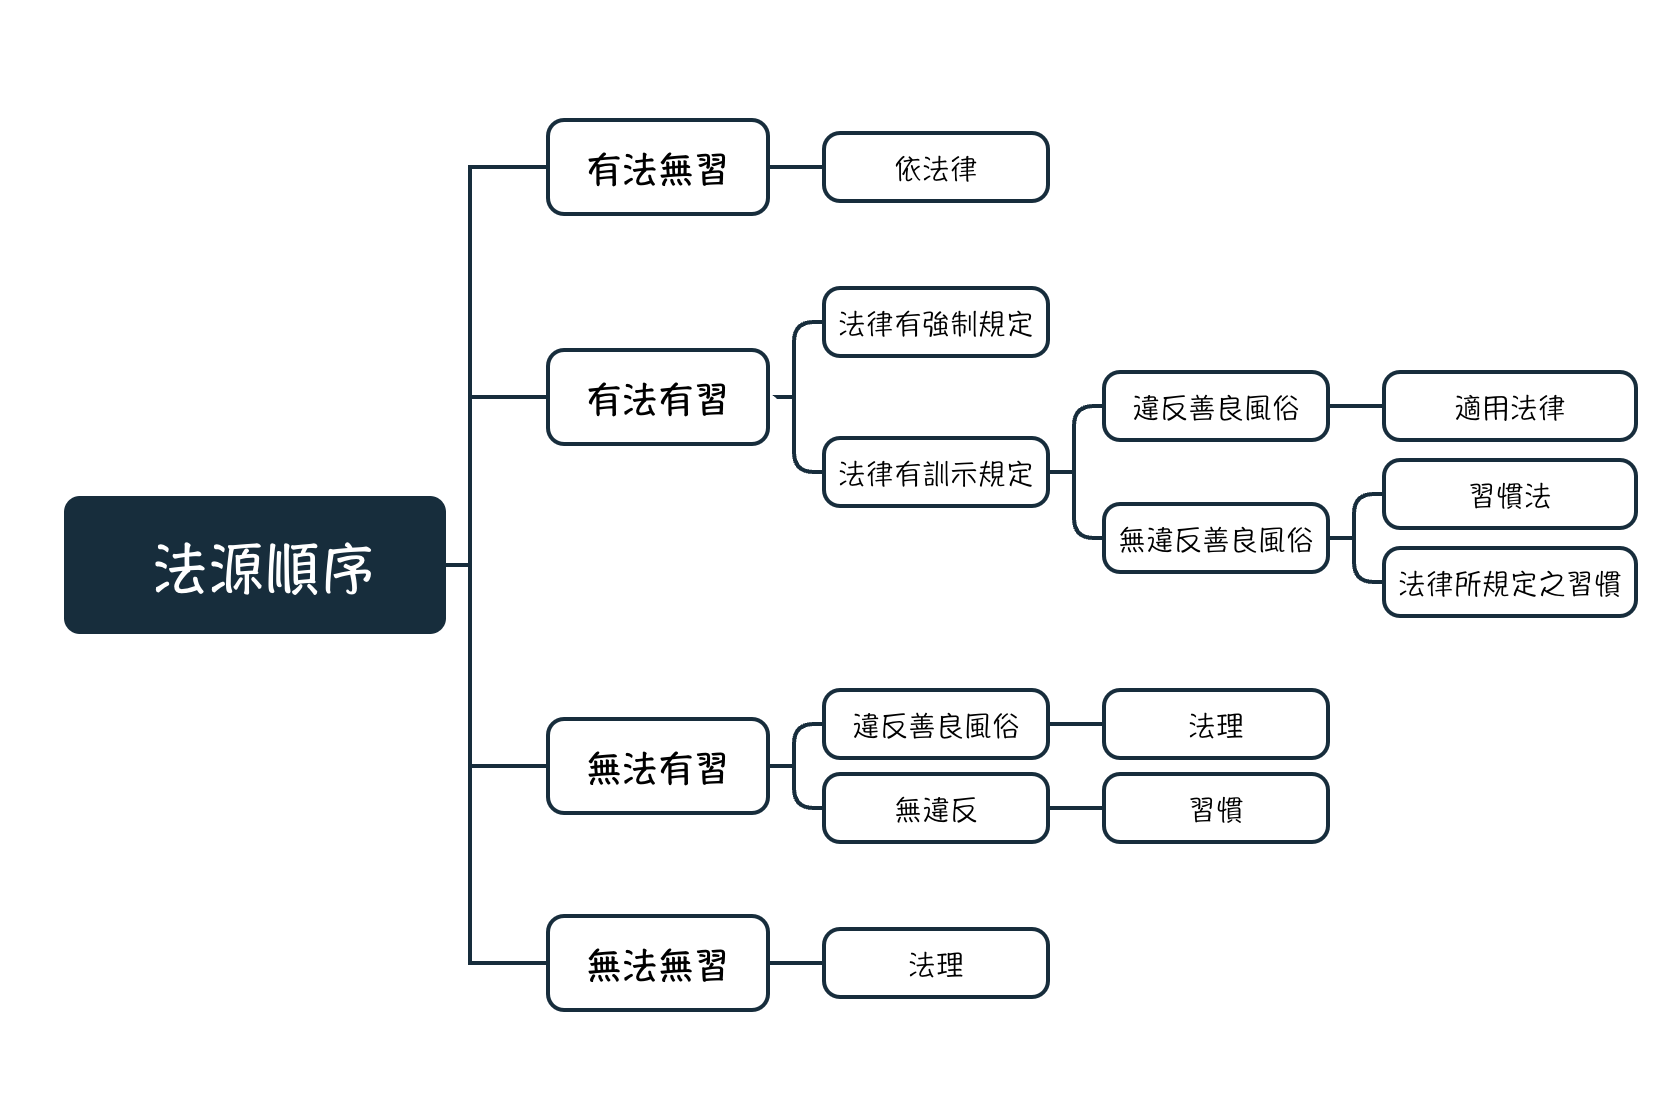
\includegraphics[width=0.8\linewidth]{www/法源適用}

\hypertarget{ux6c11ux6cd512}{%
\subsection{\texorpdfstring{\href{https://law.moj.gov.tw/LawClass/LawAll.aspx?pcode=B0000001}{民法1、2}}{民法1、2}}\label{ux6c11ux6cd512}}

\begin{quote}
第一條:民事,法律所未規定者,依習慣;無習慣者,依法理。
第二條:民事所適用之習慣,以不背於公共秩序或善良風俗者為限。
\end{quote}

\pagebreak

\hypertarget{ux6cd5ux6e90}{%
\section{法源}\label{ux6cd5ux6e90}}

\hypertarget{ux5b9aux7fa9}{%
\subsection{定義}\label{ux5b9aux7fa9}}

\begin{itemize}
\tightlist
\item
  限縮:廣義上之法律
\item
  廣義:判決之基礎-\textgreater 法律+契約(相對人中的法律)
\end{itemize}

\hypertarget{ux5ee3ux7fa9ux4e4bux6cd5ux5f8b}{%
\section{廣義之法律}\label{ux5ee3ux7fa9ux4e4bux6cd5ux5f8b}}

\hypertarget{ux6c11ux6cd5ux53caux6c11ux4e8bux7279ux5225ux6cd5}{%
\subsection{民法及民事特別法}\label{ux6c11ux6cd5ux53caux6c11ux4e8bux7279ux5225ux6cd5}}

\hypertarget{ux884cux653fux6cd5ux898f}{%
\subsection{行政法規}\label{ux884cux653fux6cd5ux898f}}

\begin{itemize}
\item
  \href{https://law.moj.gov.tw/LawClass/LawSingle.aspx?pcode=B0000001\&flno=71}{民71}:公法與私法之過度法律

  \begin{quote}
  法律行為,違反強制或禁止之規定者,無效。但其規定並不以之為無效者,不在此限。
  \end{quote}
\item
  行政法影響民法規定:\href{https://law.moj.gov.tw/LawClass/LawSingle.aspx?pcode=K0040013\&flno=15}{道交安全條例15}

  \begin{quote}
  汽車新領牌照應申請登記。
  \end{quote}

  民法之不動產無需登記
\end{itemize}

\hypertarget{ux61b2ux6cd5ux4e0dux5f97ux76f4ux63a5ux63f4ux5f15}{%
\subsection{憲法:不得直接援引}\label{ux61b2ux6cd5ux4e0dux5f97ux76f4ux63a5ux63f4ux5f15}}

\begin{itemize}
\item
  \href{https://law.moj.gov.tw/LawClass/LawSingle.aspx?pcode=B0000001\&flno=72}{民72}等過渡性法條

  \begin{quote}
  法律行為,有背於公共秩序或善良風俗者,無效。
  \end{quote}
\item
  做合憲性解釋
\end{itemize}

\hypertarget{ux570bux969bux6cd5ux8207ux81eaux6cbbux6cd5}{%
\subsection{國際法與自治法}\label{ux570bux969bux6cd5ux8207ux81eaux6cbbux6cd5}}

\pagebreak

\hypertarget{ux6cd5ux5f8bux6240ux898fux5b9aux4e4bux7fd2ux6163}{%
\subsection{法律所規定之習慣}\label{ux6cd5ux5f8bux6240ux898fux5b9aux4e4bux7fd2ux6163}}

\begin{itemize}
\item
  非指民法上之習慣,而是在法條裡有特別提及:\href{https://law.moj.gov.tw/LawClass/LawSingle.aspx?pcode=B0000001\&flno=207}{民法207}

  \begin{quote}
  利息不得滾入原本再生利息。但當事人以書面約定,利息遲付逾一年後,經催告而不償還時,債權人得將遲付之利息滾入原本者,依其約定。
  前項規定,如商業上另有習慣者,不適用之。
  \end{quote}
\end{itemize}

\hypertarget{ux7fd2ux6163ux6cd5}{%
\section{習慣法}\label{ux7fd2ux6163ux6cd5}}

\hypertarget{ux7fd2ux6163ux6cd5ux56dbux8981ux4ef6}{%
\subsection{習慣法四要件}\label{ux7fd2ux6163ux6cd5ux56dbux8981ux4ef6}}

\begin{itemize}
\item
  多年慣行之事實
\item
  普通一般人之確信心
\item
  不違背善量風俗(民2)
\item
  通常有判決加以承認
\end{itemize}

17年上字第613(已廢止)

\begin{quote}
習慣法之成立,須以多年慣行之事實及普通一般人之確信心為其基礎。
\end{quote}

\hypertarget{ux6cd5ux7406}{%
\section{法理}\label{ux6cd5ux7406}}

\hypertarget{ux4e00ux822cux6cd5ux5f8bux7684ux539fux5247}{%
\subsection{一般法律的原則}\label{ux4e00ux822cux6cd5ux5f8bux7684ux539fux5247}}

\begin{itemize}
\item
  公共利益、權利濫用、誠實信用
\item
  平等原則、舉輕明重、舉重明輕
\end{itemize}

\hypertarget{ux65b0ux5b9aux4e4bux6cd5ux5f8bux5236ux5b9aux4e2dux7684ux6cd5ux5f8bux5916ux570bux4e4bux6cd5ux5f8b}{%
\subsection{新定之法律、制定中的法律、外國之法律}\label{ux65b0ux5b9aux4e4bux6cd5ux5f8bux5236ux5b9aux4e2dux7684ux6cd5ux5f8bux5916ux570bux4e4bux6cd5ux5f8b}}

\pagebreak

\hypertarget{ux5224ux4f8bux8207ux6c7aux8b70}{%
\subsection{判例與決議}\label{ux5224ux4f8bux8207ux6c7aux8b70}}

\begin{itemize}
\tightlist
\item
  決議:最高法院及最高行政法院召開會議的方式來研討法律問題而作成的結果。
\end{itemize}

行政法院組織法第16條第3項(已廢止),目前不會再有任何決議,但可作為裁判參考

\begin{quote}
最高行政法院之裁判,其所持之法律見解,各庭間見解不一致者,於依第一項規定編為判例之前,應舉行院長、庭長、法官聯席會議,以決議統一其法律見解。
\end{quote}

\begin{itemize}
\tightlist
\item
  判例:最高法院、最高行政法院透過決議將指標性的裁判編撰而成,交給其他法院參考
\end{itemize}

\href{https://law.moj.gov.tw/LawClass/LawSingle.aspx?pcode=A0010053\&flno=57-1}{法院組織法§57條之1}

\begin{quote}
I 最高法院於中華⺠國一百零七年十二月七日本法修正施行前依法選編之判例,若無裁判全文可資查考者 ,應停止適用。
II 未經前項規定停止適用之判例,其效力與未經選編為判例之最高法院裁判相同。
\end{quote}

\hypertarget{ux5224ux6c7aux8207ux5224ux4f8bux6709ux4f55ux554fux984c}{%
\subsection{判決與判例有何問題}\label{ux5224ux6c7aux8207ux5224ux4f8bux6709ux4f55ux554fux984c}}

\begin{itemize}
\item
  判決與法例並無所謂強制之效力,但因為其為最高法院所製成,下級法官會遵循其之規定。
\item
  又依司法院釋字第374號解釋,判決與決議都可以如命令性質向大法官申請違憲審查,使其近乎有命令之地位。
\end{itemize}

如此延伸出兩種問題:

\begin{itemize}
\item
  將本質為抽象性的法規, 視為一般的抽象法規範來適用,將產生個案是否適用之疑異。
\item
  因決議與判例皆為最高法院僅透過決議而製成,又其被視為一般的抽象法規範來適用,恐有逾越司法權之虞。
\end{itemize}

\hypertarget{ux6cd5ux5f8bux9069ux7528ux7684ux610fux7fa9}{%
\section*{法律適用的意義}\label{ux6cd5ux5f8bux9069ux7528ux7684ux610fux7fa9}}
\addcontentsline{toc}{section}{法律適用的意義}

為何民法之適用有如此多的層級?其係因民事法庭不得以無法律無明文規定而拒絕審判。與此延伸出法官造法之概念

\hypertarget{ux6cd5ux5f8bux6f0fux6d1eux4e4bux627fux8a8d}{%
\subsection{法律漏洞之承認}\label{ux6cd5ux5f8bux6f0fux6d1eux4e4bux627fux8a8d}}

意義:我國乃以制定法為依據之大陸法係,立法者只能在有限法條中以抽象性的規定,盡可能涵蓋所有義務與權利關係。但條文依舊有其局限性

因此,法條之適用順序使法官得以填補法律漏洞,甚至幫助法官造法。

\hypertarget{ux6f0fux6d1eux4e4bux586bux88dc}{%
\subsection{漏洞之填補}\label{ux6f0fux6d1eux4e4bux586bux88dc}}

漏洞之種類大概分為兩種

1.依法律之規範目的,應有所規定,卻未設規定

使用類推適用,比附援引其他性質相似的法條

2.依法律之規範目的,不應有所規定,卻設有規定

使用目的性限縮解釋,排除不應適用之事項

\hypertarget{ux6709ux610fux7701ux7565}{%
\subsection{有意省略}\label{ux6709ux610fux7701ux7565}}

法律之漏洞為條文違反規定之目的,但若為立法者有意省略則非法律漏洞。

即立法者已經預先以法律規定排除適用

例:民§92-2並未如92-1就「被脅迫」而為之規定,實為立法者有意將被脅迫之情形排除再不得對抗善意第三人之列。

\begin{quote}
民§92
I:因被詐欺或被脅迫而為意思表示者,表意人得撤銷其意思表示。但詐欺係由第三人所為者,以相對人明知其事實或可得而知者為限,始得撤銷之。
II:被詐欺而為之意思表示,其撤銷不得以之對抗善意第三人。
\end{quote}

\pagebreak

\hypertarget{ux6c11ux6cd5ux4e4bux89e3ux91cb}{%
\section*{民法之解釋}\label{ux6c11ux6cd5ux4e4bux89e3ux91cb}}
\addcontentsline{toc}{section}{民法之解釋}

民法之解釋與刑法之解釋(\href{https://criminal.lsyverycute.com/司法解釋1.html}{參考})並無巨大差異,惟此章將以民法條文作為舉例。

\hypertarget{ux7acbux6cd5ux89e3ux91cb}{%
\section{立法解釋}\label{ux7acbux6cd5ux89e3ux91cb}}

立法者在法條內文中直接以明文定義,屬於立法權之展現

例:民§66、67,直接以明文方式規定何為不動產與動產

\begin{quote}
§66:
I稱不動產者,謂土地及其定著物。
II不動產之出產物,尚未分離者,為該不動產之部分。
§67:稱動產者,為前條所稱不動產以外之物。
\end{quote}

除有漏洞或矛盾,不得以約定方式推翻規定。

例:兩人共同約定土地之產出物為土地部分者,其約定無效

\hypertarget{ux53f8ux6cd5ux89e3ux91cb}{%
\section{司法解釋}\label{ux53f8ux6cd5ux89e3ux91cb}}

\hypertarget{ux7368ux7acbux89e3ux91cb}{%
\subsection{獨立解釋}\label{ux7368ux7acbux89e3ux91cb}}

為「司法院」所做出之解釋,過去的大法官制度與現行之憲法法庭均屬之。

其所做之統一解釋判決對個案與下級法院皆具有約束效力。

更詳細的憲法法庭可參考\href{https://criminal.lsyverycute.com/司法與立法解釋.html\#司法函釋司法院院字院解字-參考來源}{此章節}

\hypertarget{ux5be9ux5224ux89e3ux91cb}{%
\subsection{審判解釋}\label{ux5be9ux5224ux89e3ux91cb}}

即「最高法院」之判決,應不具有實質之拘束力,但經選為判例後,即有事實上之約束力。

雖現已不在做任何判例,但對於事實相同之個案仍有影響

\hypertarget{ux6587ux7fa9ux89e3ux91cb}{%
\section{文義解釋}\label{ux6587ux7fa9ux89e3ux91cb}}

法律解釋之起點與終點,任何解釋都不應超越其可能的文義

例:民§6(自然人)

\begin{quote}
人之權利能力,始於出生,終於死亡
\end{quote}

此處之「人」當然不包括動物(民法僅以人為主體;動物皆為客體)
而「法人」無所謂之出生與死亡,固不適用本條

但法律之解釋亦不應拘泥於文字本身

例:民§68-2之「處分」僅為法律上之負擔行為
與民§84之「處分」兼具有負擔與處分兩者之性質不同

\begin{quote}
民§68-2:主物之處分,及於從物。
民§84:法定代理人允許限制行為能力人處分之財產,限制行為能力人,就該財產有處分之能力。
\end{quote}

而在文義可能之範圍做出解釋可能有以下之「結果」

\hypertarget{ux64f4ux5f35ux89e3ux91cb}{%
\subsection{擴張解釋}\label{ux64f4ux5f35ux89e3ux91cb}}

將法條之文字採取廣義之意義

例:民§1(法源適用順序),將「法律」採取廣義之概念,擴及法律與命令。

\begin{quote}
民事,法律所未規定者,依習慣;無習慣者,依法理。
\end{quote}

\hypertarget{ux9650ux7e2eux89e3ux91cb}{%
\subsection{限縮解釋}\label{ux9650ux7e2eux89e3ux91cb}}

依法律之精神與目的,將文義加以限縮

例:民§125(請求權消滅時效),排除人格與身份之請求權

\begin{quote}
請求權,因十五年間不行使而消滅。但法律所定期間較短者,依其規定。
\end{quote}

\hypertarget{ux53cdux5c0dux89e3ux91cb}{%
\subsection{反對解釋}\label{ux53cdux5c0dux89e3ux91cb}}

使用反推論,依照文義解釋推論其反面之結果

例:民§12(成年),未滿18歲及為未成年

\begin{quote}
滿十八歲為成年。
\end{quote}

並非所有條文皆能使用反對解釋,必須要法律要件與效果具有強烈的相關性,且要件充分列舉。

例:民§17-2(自由之限制),不得解釋為「自由以外之權利限制得以違背公共秩序或善良風俗」

\begin{quote}
自由之限制,以不背於公共秩序或善良風俗者為限。
\end{quote}

\hypertarget{ux7576ux7136ux89e3ux91cb}{%
\subsection{當然解釋}\label{ux7576ux7136ux89e3ux91cb}}

法律無明文規定,但衡諸事理,認為某種事項當然包括在內

最常見的形式包括舉重明輕與舉輕明重

限制之規定多有舉輕明重,例:民§20-2(住居限制),更嚴重之3住居當然在禁止之列。

\begin{quote}
一人同時不得有兩住所。
\end{quote}

賦予權利多見舉重明輕

\hypertarget{ux8ad6ux7406ux89e3ux91cb}{%
\section{論理解釋}\label{ux8ad6ux7406ux89e3ux91cb}}

不以法律所規定之文字,而從其精神、目的、立法背景等闡明法律之含義。

\hypertarget{ux9ad4ux7cfbux89e3ux91cb}{%
\subsection{體系解釋}\label{ux9ad4ux7cfbux89e3ux91cb}}

將法律當作一個整體,在法條所在之篇章體系以及法律位階加以解釋,需注意:

\begin{itemize}
\item
  維護法律用語統一性,相同概念做相同解釋
\item
  使下位階層與上位之規範不互相矛盾
\end{itemize}

\hypertarget{ux6b77ux53f2ux89e3ux91cb}{%
\subsection{歷史解釋}\label{ux6b77ux53f2ux89e3ux91cb}}

參酌立法史與立法資料,探尋立法者主觀之意思。

越近之立法解釋越值得參考,反之,古老之法律多以與制定者分離,適應現代社會而有所改變。

\hypertarget{ux6bd4ux8f03ux6cd5ux89e3ux91cb}{%
\subsection{比較法解釋}\label{ux6bd4ux8f03ux6cd5ux89e3ux91cb}}

參酌外國立法例及判例、學說

\hypertarget{ux76eeux7684ux89e3ux91cb}{%
\subsection{目的解釋}\label{ux76eeux7684ux89e3ux91cb}}

從客觀之角度探求法律之規範目的與意義,固必須探討多個層面

\hypertarget{ux6b0aux5229ux4e3bux9ad4}{%
\chapter{權利主體}\label{ux6b0aux5229ux4e3bux9ad4}}

\hypertarget{ux6587ux5b57ux8207ux6578ux91cf}{%
\chapter{文字與數量}\label{ux6587ux5b57ux8207ux6578ux91cf}}

\hypertarget{ux79c1ux6cd5ux95dcux4fc2ux57faux672cux7d50ux69cb}{%
\chapter{私法關係基本結構}\label{ux79c1ux6cd5ux95dcux4fc2ux57faux672cux7d50ux69cb}}

\hypertarget{ux95dcux4fc2ux7d50ux69cb}{%
\section{關係結構}\label{ux95dcux4fc2ux7d50ux69cb}}

\begin{itemize}
\item
  意義:由民事法行成、規範並能藉由其實現
\item
  內容:權利之得喪變更,至少一個權利為要素
\item
  變動:基本由當事人自由約定,例外加以限制。
\end{itemize}

x

債權

物權

人格權

身份權

定義

請求特定人為給付、不給付

直接、排他性的支配標的物

禁止他人侵害擠身人格尊嚴

享受身份關係確保之權利

財產權

否

否

是

是

對世性

相對權

絕對權

絕對權

絕對權

\begin{itemize}
\item
  財產權之特性:得轉移、繼承,又稱一生專屬性
\item
  對世性之特性:得以向第三主張權利內容。
\end{itemize}

x

物權

債權

定義

直接支配具排他性

只存在特定人之間的權利

取得

原始取得繼受

意定:契約153
法定:無因(172)、不當(179)、侵權(184)

消滅

讓與、拋棄他人善意取得侵權破壞

債務清償

變更

附合共有變更權利範圍

債務物權化主、客、內容變更

\hypertarget{ux50b5ux6b0aux7269ux6b0aux5316ux8cb7ux8ce3ux4e0dux7834ux79dfux8cc3}{%
\section{債權物權化:買賣不破租賃}\label{ux50b5ux6b0aux7269ux6b0aux5316ux8cb7ux8ce3ux4e0dux7834ux79dfux8cc3}}

某甲與某乙締結租屋契約(\href{https://law.moj.gov.tw/LawClass/LawSingle.aspx?pcode=B0000001\&flno=421}{421}),雙方產生債權權。再契約尚未結束前,將房屋所有權讓與某丙(\href{https://law.moj.gov.tw/LawClass/LawSingle.aspx?pcode=B0000001\&flno=758}{758})(\href{https://law.moj.gov.tw/LawClass/LawSingle.aspx?pcode=B0000001\&flno=345}{345}),丙持有房屋的物權。此時,丙不得以物上返還權(\href{https://law.moj.gov.tw/LawClass/LawSingle.aspx?pcode=B0000001\&flno=767}{767})將某乙趕出,租賃之契約依然有效。及買賣不破租賃。

\begin{quote}
民法§425 第 1 項:「出租人於租賃物交付後,承租人占有中,縱將其所有權讓與第三人,其租賃契約,對於受讓人仍繼續存在。」
\end{quote}

\hypertarget{ux6b0aux5229ux5ba2ux9ad4ux4ee5ux7269ux70baux4e2dux5fc3}{%
\chapter{權利客體―以「物」為中心}\label{ux6b0aux5229ux5ba2ux9ad4ux4ee5ux7269ux70baux4e2dux5fc3}}

\hypertarget{ux6b0aux529bux7684ux57faux672cux6982ux5ff5}{%
\section{權力的基本概念}\label{ux6b0aux529bux7684ux57faux672cux6982ux5ff5}}

權利

權利主體

權利客體

享受特定利益的力量

得享有權利者
(擁有權利能力者)

權利支配的對象

\hypertarget{ux7269ux6b0aux7684ux57faux672cux539fux5247ux4e00ux7269ux4e00ux6b0a}{%
\section{物權的基本原則:一物一權}\label{ux7269ux6b0aux7684ux57faux672cux539fux5247ux4e00ux7269ux4e00ux6b0a}}

\begin{itemize}
\item
  一個物權支配一個特定的物

  例:書包中的民法總則,刑法總則與小六法共有三個所有權
\item
  物權抽象,物是具體的

  不代表無體物不是物
\item
  以法律行為使權力發生變動時,是物權改變

  例:買一隻羊,不是羊此物發生改變,是的物權改變
\end{itemize}

\pagebreak

\hypertarget{ux7269ux7684ux5224ux65b7}{%
\section{物的判斷:}\label{ux7269ux7684ux5224ux65b7}}

\hypertarget{ux4e0dux4ee5ux6709ux9ad4ux7269ux70baux9650ux4ea6ux53efux70baux7121ux9ad4ux7269}{%
\subsection{1.不以有體物為限,亦可為無體物}\label{ux4e0dux4ee5ux6709ux9ad4ux7269ux70baux9650ux4ea6ux53efux70baux7121ux9ad4ux7269}}

有體物

無體物

外觀上具備一定之形體

沒有一定之形體

車子、房屋、羊

氣體、液體、電力

\hypertarget{ux7279ux4f8bux8a0eux8ad6ux96fbux5b50ux6a94ux6848ux662fux5426ux70baux7269}{%
\subsection{特例討論:電子檔案是否為物?}\label{ux7279ux4f8bux8a0eux8ad6ux96fbux5b50ux6a94ux6848ux662fux5426ux70baux7269}}

\begin{itemize}
\tightlist
\item
  正方:從權利主體的保護利義論
\end{itemize}

將其納入物的範圍,使其能成為侵權行為之客體。例如將他人之電子檔案以木馬病毒摧毀。

\begin{itemize}
\tightlist
\item
  反方:比照德國法,採有體物之觀念
\end{itemize}

電子檔案僅屬於精神之產物(類無體財產權),但其交易仍可依435條準用物之買賣或租賃之規定

\hypertarget{ux53efux53d7ux4ebaux985eux652fux914d}{%
\subsection{2.可受人類支配}\label{ux53efux53d7ux4ebaux985eux652fux914d}}

\begin{itemize}
\item
  特指具排他性的支配,物權得直接支配標的物

  \begin{itemize}
  \item
    支配:是指依權利人之意思,對物管領處分。例外:愛情、時間、資訊不能被支配。
  \item
    直接:支配標的物時,他人之意思或行為不能介入。
    例外資訊、知識等不能防止獲取。(但仍可以無體財產權的形式保護)。
  \end{itemize}
\end{itemize}

\hypertarget{ux975eux4ebaux683cux6027}{%
\subsection{3.非人格性}\label{ux975eux4ebaux683cux6027}}

\begin{itemize}
\item
  因人為權利主體,人之身體乃人格權的一部分
\item
  但離開身體之器官、頭髮等依然可以為物

  \begin{itemize}
  \item
    其為不通融物,即不可交易買賣(民72)
  \item
    僅得在一定條件下贈與(人體器官移植條例6)
  \end{itemize}
\end{itemize}

\pagebreak

\hypertarget{ux9aa8ux7070ux5c4dux9ad4ux4f7fux5426ux70baux7269}{%
\subsection{骨灰、屍體使否為物}\label{ux9aa8ux7070ux5c4dux9ad4ux4f7fux5426ux70baux7269}}

\begin{itemize}
\item
  屍體:多數學說認為屍體為物,構成遺產,應為繼承人所公同共有, 其所有權內涵與其他財產權之所有權不同,應以屍體之埋葬、管理、祭祀及供養為目的,不得自由使用、收益及處分,拋棄繼承之效力不及於此。
\item
  骨灰:與屍體類型相似,使用統一解釋
\item
  身體之人工部分:恢復最原始物之狀態,其是否分離因由繼承者決定,由繼承者獲得處分權
\item
  木乃伊或骷髏:得為權利客體
\end{itemize}

\href{\%22https://tyd.judicial.gov.tw\%22}{臺灣桃園地方法院92年度國字第4號判決}

\begin{quote}
骨灰是否為物,法無明文,惟參酌多數學說認為屍體為物,構成遺產,應為繼承人所公同共有, 其所有權內涵與其他財產權之所有權不同,應以屍體之埋葬、管理、祭祀及供養為目的,不得自由 使用、收益及處分,本院認骨灰性質與屍體相近,應作同一解釋較符法理及我國社會上一般觀念。 故被告抗辯本件原告主張寄放於納骨塔之骨灰應屬原告及其他繼承人所繼承遺產之一部,屬全體繼 承人公同共有乙節,應屬可採。
\end{quote}

\hypertarget{ux5b58ux5728ux7368ux7acbux6027}{%
\subsection{4.存在獨立性}\label{ux5b58ux5728ux7368ux7acbux6027}}

\begin{itemize}
\item
  必須存在一定之空間、範圍
  clear
  流動的河流,空中的閃電
  check
  經過登記後的不動產
\item
  必須獨立個必存在,數物之重要成份而不得分離者,不得作為物權之客體,即一物一權
  clear
  土地上之樹木之果實(但得作為買賣之標的)
\end{itemize}

\hypertarget{ux53efux6effux8db3ux4ebaux985eux751fux6d3bux6240ux9700}{%
\subsection{5.可滿足人類生活所需}\label{ux53efux6effux8db3ux4ebaux985eux751fux6d3bux6240ux9700}}

\begin{itemize}
\tightlist
\item
  必須對人類生活有特殊意義或功能
  clear
  一粒米、湖裡之微生物
  check
  雕刻過的米、專供研究而培養成的微生物
\end{itemize}

\pagebreak

\hypertarget{ux7269ux7684ux7a2eux985e}{%
\section{物的種類}\label{ux7269ux7684ux7a2eux985e}}

\hypertarget{ux52d5ux7522ux8207ux4e0dux52d5ux7522}{%
\subsection{1.動產與不動產}\label{ux52d5ux7522ux8207ux4e0dux52d5ux7522}}

\hypertarget{ux5340ux5225ux6a19ux6e96}{%
\subsection{區別標準}\label{ux5340ux5225ux6a19ux6e96}}

\href{https://law.moj.gov.tw/LawClass/LawSingle.aspx?pcode=B0000001\&flno=66}{民66:不動產}

\begin{quote}
1.稱不動產者,謂土地及其定著物。
2.不動產之出產物,尚未分離者,為該不動產之部分。
\end{quote}

\begin{itemize}
\tightlist
\item
  定著物定義
\end{itemize}

最高法院63年第六次民庭庭推總會議決議(一)

\begin{quote}
民法第六十六條第一項所謂定著物,係指非土地之構成部分,繼續附著於土地,而達一定經濟上目的,不易移動其所在之物而言。凡屋頂尚未完全完工之房屋,其已足避風雨,可達經濟上使用之目的者,即屬土地之定著物,買受此種房屋之人,乃係基於法律行為,自須辦理移轉登記,始能取得所有權。
\end{quote}

\begin{itemize}
\tightlist
\item
  爛尾樓,違建:皆符合
\end{itemize}

\href{https://cons.judicial.gov.tw/docdata.aspx?fid=100\&id=310274}{釋字93號}

\begin{itemize}
\tightlist
\item
  輕便軌道:符合
\end{itemize}

\begin{quote}
輕便軌道除係臨時敷設者外,凡繼續附著於土地而達其一定經濟上之目的者,應認為不動產。
\end{quote}

\href{https://law.moj.gov.tw/LawClass/LawSingle.aspx?pcode=B0000001\&flno=67}{民67:動產}

\begin{quote}
稱動產者,為前條所稱不動產以外之物。
\end{quote}

\hypertarget{ux5340ux5225ux5be6ux76caux6240ux6709ux6b0aux6b0aux5229ux8b8aux52d5ux4e4bux65b9ux6cd5ux4e0dux540c}{%
\subsection{區別實益:所有權權利變動之方法不同}\label{ux5340ux5225ux5be6ux76caux6240ux6709ux6b0aux6b0aux5229ux8b8aux52d5ux4e4bux65b9ux6cd5ux4e0dux540c}}

\href{https://law.moj.gov.tw/LawClass/LawSingle.aspx?pcode=B0000001\&flno=67}{民758:不動產必須要書面登記}

\begin{quote}
1.不動產物權,依法律行為而取得、設定、喪失及變更者,非經登記,不生效力。
2.前項行為,應以書面為之。
\end{quote}

為何違章建築、爛尾樓難以處理=\textgreater 成為未登記之不動產,亦難以轉移,變更

\hypertarget{ux4f55ux70baux6b0aux5229ux8b8aux52d5}{%
\chapter{何為權利變動}\label{ux4f55ux70baux6b0aux5229ux8b8aux52d5}}

\begin{itemize}
\item
  定義:基於一定的法律事實,產生權利得喪變更的法律效果
\item
  特性:債權、物權為主
\item
  基本原則:私法自治、契約自由
\item
  意思:形成法律關係:

  \begin{itemize}
  \item
    基於當事人之意思形成其關係:契約(私法自治)
  \item
    非,由法律擬制(偏離原則)
  \end{itemize}
\end{itemize}

\hypertarget{ux6848ux4f8bux3127ux7269ux4e8cux8ce3}{%
\section{案例:ㄧ物二賣}\label{ux6848ux4f8bux3127ux7269ux4e8cux8ce3}}

甲與乙依民§345將持有之房屋賣與乙,而後又與丙締結買賣契約

1、甲乙間約定效果為何?

2、誰是不動產的所有權人?

\hypertarget{ux50b5ux6b0aux4e4bux5951ux7d04ux6c11345}{%
\subsection{債權之契約:民§345}\label{ux50b5ux6b0aux4e4bux5951ux7d04ux6c11345}}

\begin{quote}
1.稱買賣者,謂當事人約定一方移轉財產權於他方,他方支付價金之契約。
當事人就標的物及其價金互相同意時,買賣契約即為成立。
\end{quote}

是一種雙物契約
負擔行為、債權行為
甲移轉財產權給乙=乙向甲請求轉移
乙支負債金=甲向乙請求價金

雙方藉由意思表示(締結契約:債權行為)而由民§345之法律效果產生兩個債權

債權行為不會產生其他法律效果(物權變動)

\hypertarget{ux7269ux6b0aux4e4bux5951ux7d04ux6c11761-1}{%
\subsection{\texorpdfstring{物權之契約:\href{https://law.moj.gov.tw/LawClass/LawSingle.aspx?pcode=B0000001\&flno=761}{民§761-1}}{物權之契約:民§761-1}}\label{ux7269ux6b0aux4e4bux5951ux7d04ux6c11761-1}}

\begin{quote}
1.動產物權之讓與,非將動產交付,不生效力。但受讓人已占有動產者,於讓與合意時,即生效力。
\end{quote}

\begin{itemize}
\item
  讓與合意(對物權之變動達成合議):基於雙方之意思而產生之法律效果=\textgreater 物權行為,而非行成債權
  物權之讓與合意也是契約,此契約產生物之權利之變動
\item
  交付(標的物之所有權)
  不以意思作為要素,而是客觀之事實,法律擬制其效果
  換句話說,交付之意思有無、背後原因為何,不影響交付之發生
\end{itemize}

\hypertarget{ux7d50ux8ad6}{%
\subsection{結論:}\label{ux7d50ux8ad6}}

1.甲與乙、丙買賣契約僅限與債權債務之產生,不會產生物權(所有權)之變動

2.物權之變動必須有物權行為(契約)並且有法定方法,因此房屋之物權仍為甲所有

\hypertarget{ux6cd5ux5f8bux4e8bux5be6}{%
\section{法律事實}\label{ux6cd5ux5f8bux4e8bux5be6}}

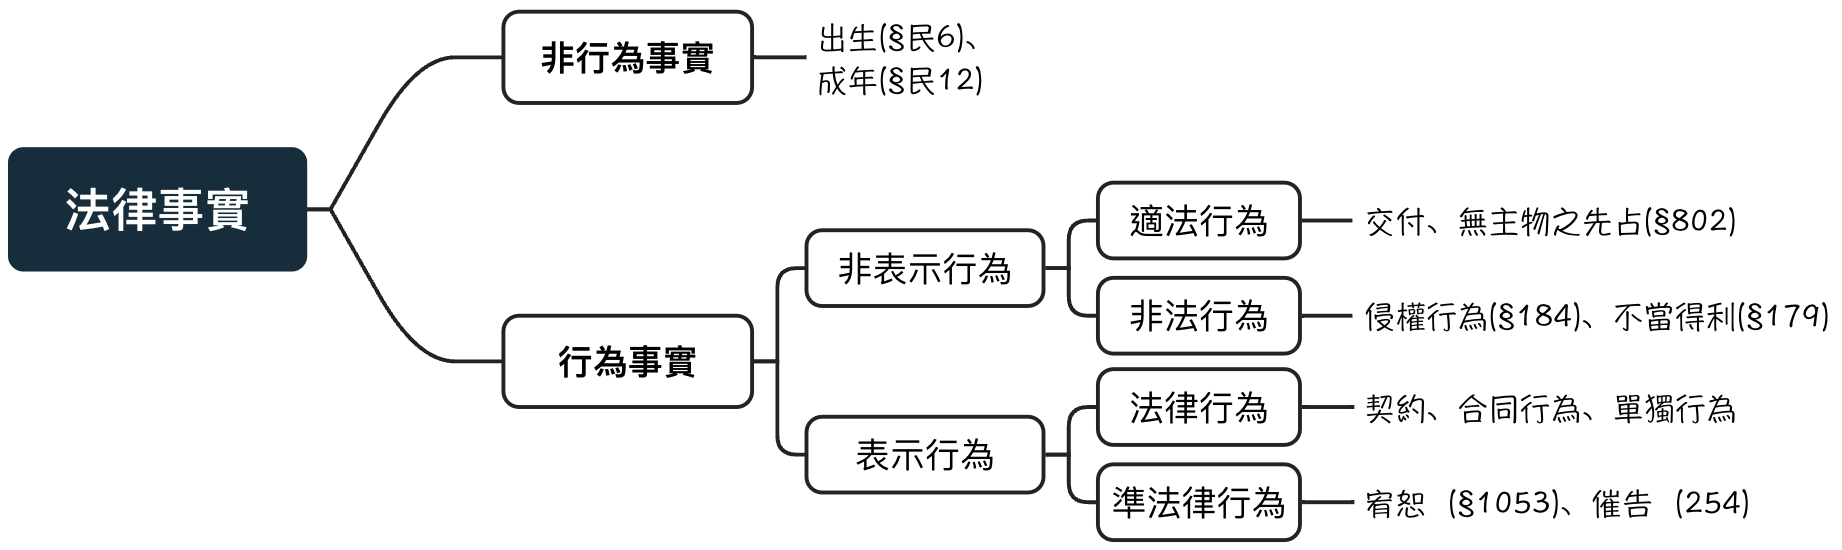
\includegraphics[width=0.8\textwidth,height=\textheight]{www/權利變動1.png}

\hypertarget{ux6cd5ux5f8bux4e8bux5be6ux4e4bux5206ux985e}{%
\subsection{法律事實之分類}\label{ux6cd5ux5f8bux4e8bux5be6ux4e4bux5206ux985e}}

\begin{itemize}
\item
  法律事實:
  定義:能夠與權利與義務相關聯的事實
  反例:睡覺、吃飯
\item
  行為與非行為事實

  \begin{itemize}
  \item
    行為事實:經由人的行為所發生者
  \item
    非行為事實:非經由人的行為所發生者
    例:出生(§民6)、成年(§民12)
  \end{itemize}
\item
  適法行為:

  \begin{itemize}
  \item
    法律行為:以\textbf{意思表示}為主體,透過將意思表露於外,法律之規定賦予相符合之法律效果
    最典型的契約,另有單獨行為(例:遺囑)、合同行為(例:創立社團法人)
    契約又可分為1.債務契約 2.物權契約
  \item
    準法律行為:\textbf{意思通知、觀念通知、感情表示}
    得類推適用法律行為之規定(例:得有漏洞之填補)
    例:催告(254, 無須針對金額有所認識)、觀念通知(股東會召集)、宥恕(§1053;原諒=\textgreater 喪失請求權)
  \end{itemize}
\item
  事實行為(法定之債):基於事實上的行為而\textbf{非以意思或精神表示}為要素
  無涉及行為人內心意思表示,與法律行為類型不同,無類推適用

  \begin{itemize}
  \item
    適法行為:無主物之先占(§802),埋藏物之發現(§808)
  \item
    非法行為:侵權行為(§184)、不當得利(§179)
  \end{itemize}
\end{itemize}

\hypertarget{ux6cd5ux5f8bux884cux70ba}{%
\section{法律行為}\label{ux6cd5ux5f8bux884cux70ba}}

\begin{itemize}
\item
  物權與債權行為之分類

  \begin{itemize}
  \item
    負擔行為:發生債權債務為其內容的法律行為,亦稱「債權行為」
  \item
    處分行為:直接使權利發生、變更或消滅的行為,包含「物權行為」與「準物權行為」

    \begin{itemize}
    \item
      物權行為:發生物權法上效果之行為,如物權之讓與合意(物權契約)
    \item
      準物權行為:使物權以外之權利發生、變更或消滅之行為。如債務免除、債權讓與、股份讓與
    \end{itemize}
  \end{itemize}
\end{itemize}

  \bibliography{book.bib,packages.bib}

\end{document}
